\documentclass[usenames,dvipsnames, 18pt, compress, aspectratio=169]{beamer}

% can be compiled by xelatex -shell-escape presentation.tex
% lualatex -shell-escape presentation.tex

\usetheme[]{metropolis}

\usepackage[utf8]{inputenc}
\usepackage[russian, english]{babel}
\usepackage{booktabs}
\usepackage[scale=2]{ccicons}
\usepackage{listings}
\usepackage{marvosym}
\usepackage{color}
\usepackage{xcolor}
\usepackage[document]{ragged2e}
\usepackage[export]{adjustbox}
\usepackage{fontawesome}
\usepackage{enumitem}
\usepackage{minted}
\usemintedstyle{tango}
\usepackage[normalem]{ulem}
\usepackage{tikz}
\usetikzlibrary{patterns}
\usetikzlibrary{mindmap}
\usetikzlibrary{shapes.misc, fit}
\usepackage{graphicx}
\usepackage{eso-pic}
\usepackage{verbatim}
\usepackage{smartdiagram}
\usesmartdiagramlibrary{additions}
\usetikzlibrary{trees}
\usepackage{datetime}
\usepackage{hyperref}
\usepackage{forloop}
\usepackage{csquotes}
\usetikzlibrary{tikzmark}
\usetikzlibrary{arrows.meta}

\usepackage{tcolorbox}
\usepackage{tabularx}
\usepackage{array}
\usepackage{colortbl}
\tcbuselibrary{skins}

\usetikzlibrary{shapes,arrows,positioning}
\graphicspath{{images/}}
\newfontfamily{\FA}{FontAwesome}

\def\twitter{{\FA \faTwitter}}
\def\github{{\FA \faGithub}}
\def\email{{\FA \faEnvelope}}

\renewcommand{\ttdefault}{pcr}
\newfontfamily{\ttfamily}{Fira Code}

\usefonttheme{professionalfonts} % using non standard fonts for beamer
\usefonttheme{serif} % default family is serif
\usepackage{fontspec}
\setmainfont{Liberation Sans}
\newfontfamily\ExtraLight{Liberation Sans}
\newfontfamily\Light{Liberation Sans}
\newfontfamily\Book{Liberation Sans}
\newfontfamily\Medium{Liberation Sans}

\makeatletter
\newcommand\HUGE{\@setfontsize\Huge{32}{41}}
\makeatother

\newcommand\AtPagemyUpperLeft[1]{\AtPageLowerLeft{%
\put(\LenToUnit{0.85\paperwidth},\LenToUnit{0.05\paperheight}){#1}}}

\newcommand\AtPagemyUpperTop[1]{\AtPageLowerLeft{%
\put(\LenToUnit{0.42\paperwidth},\LenToUnit{0.90\paperheight}){#1}}}

\renewcommand{\ULthickness}{2.0pt}

\definecolor{links}{HTML}{0099FF}
\hypersetup{colorlinks, linkcolor=, urlcolor=links}
\definecolor{greenGood}{HTML}{99FF99}
\definecolor{redBad}{HTML}{FF9980}

\setbeamerfont{section title}{family=\Book, size=\Huge, shape=\normalfont}
\setbeamerfont{frametitle}{family=\Book, size=\large, shape=\normalfont}
\setbeamerfont{title}{family=\Book, size=\Large, shape=\normalfont}
\setbeamerfont{subtitle}{size=\small}
\setbeamerfont{author}{family=\ExtraLight, size=\footnotesize}

\definecolor{cec1d24}{RGB}{236,29,36}
\definecolor{cffffff}{RGB}{255,255,255}

\pagenumbering{gobble}

\newdateformat{specialdate}{\twodigit{\THEDAY}-\twodigit{\THEMONTH}-\THEYEAR}

\def\strongdata{strong_correlation.data}
\def\weakdata{weak_correlation.data}

\setbeamertemplate{title page}
{

  \vspace*{2.1cm}
  \begin{minipage}[b][\paperheight]{\textwidth}
  \begin{center}

    \ifx\inserttitle\@empty\else
    {{% \inserttitle is nonempty
      \raggedright%
      %\linespread{1.0}%
      \usebeamerfont{title}%
      \usebeamercolor[fg]{title}%
      %\vspace*{1.3em}
      \if@noSmallCapitals%
        \inserttitle%
      \else%
        \scshape{\color{black} \textbf{\begin{center}\inserttitle\end{center}}}%
      \fi%
      \vspace*{0.3em}
    }}
    \fi

    \vspace*{0.5em}%

    \ifx\insertsubtitle\@empty\else
    {{% \insertsubtitle is nonempty
      \usebeamerfont{subtitle}%
      \usebeamercolor[fg]{subtitle}%
      {\color{black} \insertsubtitle}%
      \vspace*{3.0em}%
    }}
    \fi

    \vspace*{1.0em}%

    \usebeamerfont{author}%
    \usebeamercolor[fg]{author}%
    {\color{black} \insertauthor}%

    \vspace*{1.5em}
    \fontsize{8pt}{10}\selectfont
    {\color{black} 31-01-2020}%

    \vfill
    \vspace*{2em}
  \end{center}
  \end{minipage}
}

\setbeamertemplate{section page}
{
  \vspace{2em}
  \centering
  \begin{minipage}{22em}
    \usebeamercolor[fg]{section title}
    \usebeamerfont{section title}
    {\color{black} \insertsectionhead\\[-1ex]}
  \end{minipage}
  \par
}

\setbeamertemplate{footline}
{
\begin{beamercolorbox}[wd=\textwidth,ht=3ex,dp=3ex,leftskip=0.3cm,rightskip=0.3cm]{structure}
  \usebeamerfont{page number in head/foot}
  \insertframenumber
\end{beamercolorbox}
}

\title{Sounds of \\ Open Source}
\subtitle{processing sound with sox}
\date{\today}
\author{DMITRY DOLGOV}
\institute{}

\begin{document}
{
  \usebackgroundtemplate{
\includegraphics[width=\paperwidth]{template_2.png}}%
  \fontsize{17pt}{18}\selectfont
  \maketitle
}

\AddToShipoutPictureBG{
  \AtPagemyUpperLeft{{
\includegraphics[width=2.0cm,keepaspectratio]{logo.png}}}
}%

\setbeamertemplate{background canvas}{
\begin{tikzpicture}
    \clip (0,0) rectangle (\paperwidth,\paperheight);
    \fill[color=orange] (4cm, \paperheight-6pt) rectangle (\paperwidth-4cm,\paperheight);
\end{tikzpicture}
}

\begin{frame}
    \frametitle{}
    \begin{center}
        
\includegraphics[width=0.5\textwidth,center]{swiss_knife.png}
        \vspace{-0.8cm}
        \hspace*{6cm}
        \href{https://freesvg.org/by/OpenClipart}
             {\color{black}\fontsize{5pt}{0}\selectfont @OpenClipart}

    \end{center}
\end{frame}

\begin{frame}[fragile]{}
    \frametitle{}
    \begin{center}
        \textbf{Record audio}
        \vspace{0.2cm}

        \begin{minted}[fontsize=\normalsize]{bash}
    rec -r 44100 -b 16 -e signed-integer audio.mp3
        \end{minted}

    \end{center}
\end{frame}

\begin{frame}[fragile]{}
    \frametitle{}
    \begin{center}
        \textbf{Record audio}
        \vspace{0.2cm}

        \begin{minted}[fontsize=\normalsize]{bash}
    # Thread_queue_size applies to the first
    # input specified after it.
    # In some cases it's not enough to avoid
    # "buffer xrun", try to record video and
    # audio separately.

    ffmpeg -f alsa -thread_queue_size 4096
        -i hw:0 -acodec aac audio.mp3
        \end{minted}

    \end{center}
\end{frame}

\begin{frame}[fragile]{}
    \frametitle{}
    \begin{center}
        \textbf{Record audio}
        \vspace{0.2cm}

        %\vspace{-0.5cm}
        \begin{itemize}[label={\MVRightarrow}]
            \item Self-describing formats\\
                \vspace{0.5cm}
                \hspace{2cm}
                \begin{minipage}[b]{0.6\linewidth}
                    
\includegraphics[width=0.2\textwidth]{wav_logo.png}
                    \hfill
                    
\includegraphics[width=0.2\textwidth]{mp3_logo.png}
                    \hfill
                    
\includegraphics[width=0.2\textwidth]{flac_logo.png}
                \end{minipage}
                \vspace{0.5cm}
            \item Raw or headerless formats\\
                \vspace{0.5cm}
                \hspace{2cm}
                \begin{minipage}[b]{0.6\linewidth}
                    
\includegraphics[width=0.2\textwidth]{binary_logo.png}
                \end{minipage}
        \end{itemize}

    \end{center}
\end{frame}
\note{
    \begin{itemize}
    \item WAV, uncompressed audio in the linear pulse-code modulation (LPCM) format
    \item FLAC, lossless compression, linear prediction and run-length encoding
    \item MP3, lossy data-compression to encode data using inexact approximations and the partial discarding of data
    \end{itemize}
}

%\begin{frame}[fragile]{}
    %\frametitle{}
    %\begin{center}

        %\begin{itemize}[label={\MVRightarrow}]
            %\item Self-describing formats
                %\begin{itemize}
                    %\item WAV, uncompressed audio in the linear pulse-code modulation (LPCM) format
                    %\item FLAC, lossless compression, linear prediction and run-length encoding
                    %\item MP3, lossy data-compression to encode data using inexact approximations and the partial discarding of data
                %\end{itemize}
            %\item Raw or headerless formats
        %\end{itemize}

    %\end{center}
%\end{frame}

\begin{frame}[fragile]{}
    \frametitle{}
    \begin{center}
        \textbf{Cleaning up}
        \vspace{0.2cm}

        \begin{minted}[fontsize=\normalsize]{bash}
    # the noise is always different,
    # try to record it immediately
    # before the actual audio.

    sox noise.mp3 -n noiseprof noise.prof
    sox audio.mp3 output.mp3 noisered noise.prof 0.21
        \end{minted}

    \end{center}
\end{frame}

\begin{frame}[fragile]{}
    \frametitle{}
    \begin{center}
        \textbf{Cleaning up}
        \vspace{0.2cm}

        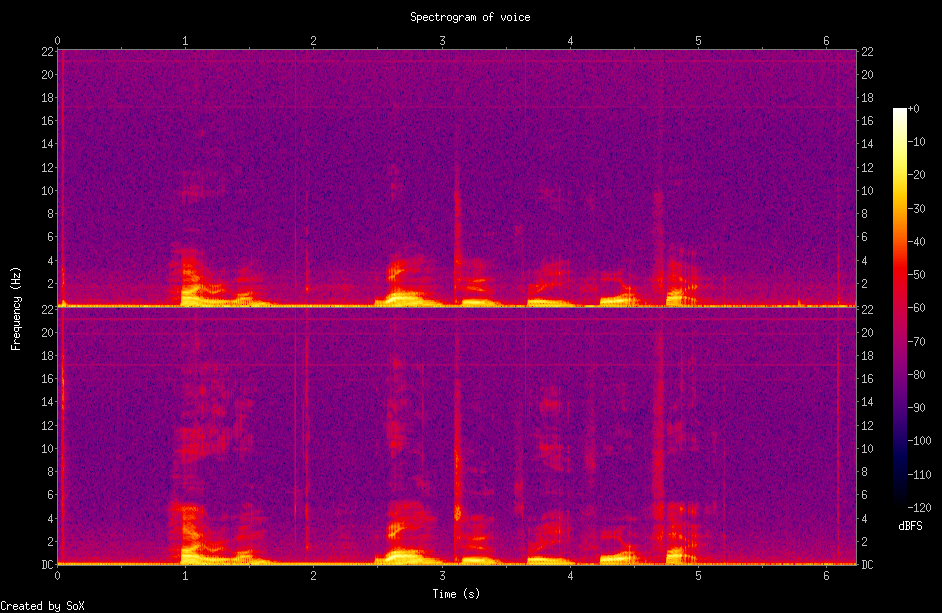
\includegraphics[width=0.48\textwidth]{voice-spectrogram.png}
        \hfill
        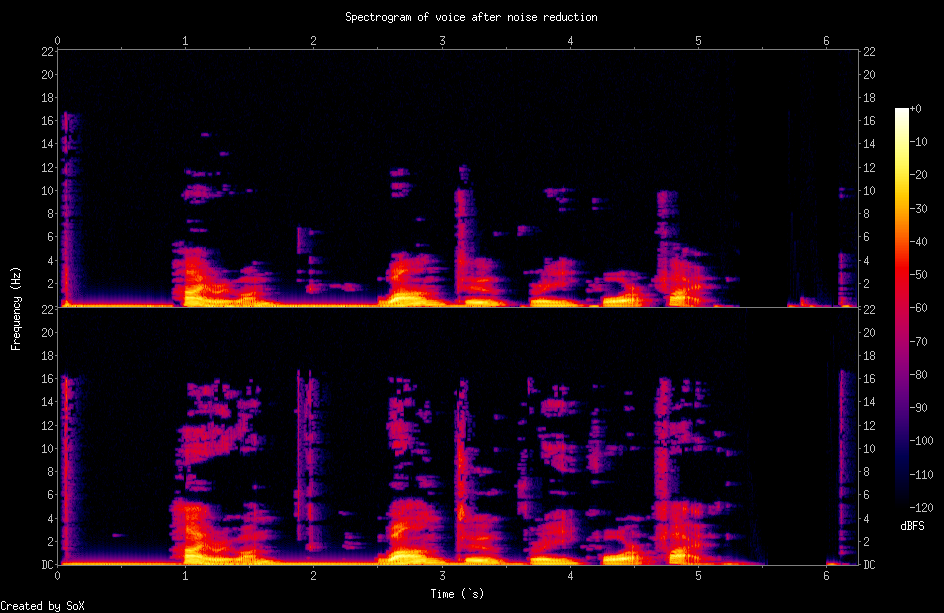
\includegraphics[width=0.48\textwidth]{voice-clean-spectrogram.png}

    \end{center}
\end{frame}

\begin{frame}[fragile]{}
    \frametitle{}
    \begin{center}
        \textbf{Cleaning up}
        \vspace{0.2cm}

        \begin{minted}[fontsize=\normalsize]{bash}
    # Voice Activity Detector to trim
    # silence and quiet background noise
    # at the beginning and the end

    sox audio.mp3 trimmed.mp3 vad

        \end{minted}

    \end{center}
\end{frame}

\begin{frame}[fragile]{}
    \frametitle{}
    \begin{center}
        \textbf{Cleaning up}
        \vspace{0.2cm}

        \begin{minted}[fontsize=\normalsize]{bash}
    # -v, --volume to adjust volume by certain factor

    sox audio.mp3 output.mp3 stat

        Samples read:            441216
        Length (seconds):     10.004898
        Scaled by:         2147483647.0
        Maximum amplitude:     0.019642
        Minimum amplitude:    -0.019630
        Mean    norm:          0.004128
        Mean    amplitude:    -0.000000
        Volume adjustment:       50.911
        \end{minted}

    \end{center}
\end{frame}

\begin{frame}[fragile]{}
    \frametitle{}
    \begin{center}
        \textbf{Automatic Gain Control}
        \vspace{0.2cm}


        \begin{minted}[fontsize=\normalsize]{bash}
    sox audio.mp3 agc.mp3 compand
        0.3,0.3 6:-80,-80,-60,-60,-40,-40,-20,-40 0 0 0.3
        \end{minted}
    \end{center}
\end{frame}

\begin{frame}[fragile]{}
    \frametitle{}
    \begin{center}
        \textbf{Automatic Gain Control}
        \vspace{0.2cm}

        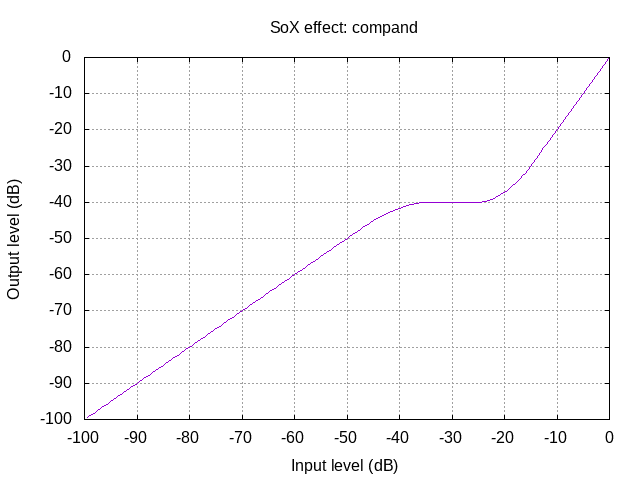
\includegraphics[width=0.7\textwidth]{agc.png}

    \end{center}
\end{frame}

\begin{frame}[fragile]{}
    \frametitle{}
    \begin{center}
        \textbf{Unite and lead}
        \vspace{0.2cm}

        \begin{minted}[fontsize=\normalsize]{bash}
    # without the volume specified sox can try to
    # automatically adjust the volume to prevent
    # clipping, making everything unexpectedly quiet.

    sox -v 1.0 part.1.mp3 part.2.mp3 concat.mp3
    sox -m -v 1.0 part.1.mp3 part.2.mp3 mixture.mp3
        \end{minted}
    \end{center}
\end{frame}

\begin{frame}[fragile]{}
    \frametitle{}
    \begin{center}
        \textbf{Unite and lead}
        \vspace{0.2cm}

        \begin{minted}[fontsize=\normalsize]{bash}
    sox audio.mp3 output.mp3 \
        trim 0 30 # cut out from the 0 to 30th second
        fade 5    # fade in/out for 5 seconds
        pad 7     # pad with 7 seconds of silence
        \end{minted}
    \end{center}
\end{frame}

\begin{frame}[fragile]{}
    \frametitle{}
    \begin{center}
        \textbf{Unite and lead}
        \vspace{0.2cm}

        \begin{minted}[fontsize=\normalsize]{bash}
    # splice two parts together at position 00:25 with
    # excess/leeway 1 second and half-cosine wave fading

    sox part1.mp3 part2.mp3 mix.mp3 \
        splice -h 00:25,1,1
        \end{minted}
    \end{center}
\end{frame}

\begin{frame}[fragile]{}
    \frametitle{}
    \begin{center}
        \textbf{Effects}
        \vspace{0.2cm}

        \begin{minted}[fontsize=\normalsize]{bash}
    # add an echo with the delay 500 ms and loudness 0.3

    sox voice.clean.mp3 echo.mp3 echo 0.8 0.9 500 0.3
        \end{minted}
    \end{center}
\end{frame}

\begin{frame}[fragile]{}
    \frametitle{}
    \begin{center}
        \textbf{Effects}
        \vspace{0.2cm}

        \begin{minted}[fontsize=\normalsize]{bash}
    # Kaiser–Bessel window band-pass filter
    # to generate "phone" effect

    sox audio.mp3 output.mp3 sinc 500-3000 vol +3

    # Add some clicking noise on top of it
    sox -n pinknoise.mp3 rate 44100 \
        synth 10 pinknoise vol 0.01
    sox -m -v 1 output.mp3 pinknoise.mp3 phone.mp3
        \end{minted}

        \href{https://en.wikipedia.org/wiki/Kaiser_window}{Kaiser-Bessel window}
    \end{center}
\end{frame}


\begin{frame}[fragile]{}
    \frametitle{}
    \begin{center}
        \textbf{Generating effects}
        \vspace{0.2cm}

        \begin{minted}[fontsize=\normalsize]{bash}
# -n says the input is a special "null" file
sox -n guitar-chortds.mp3 \

  # sine waves for tones of specified note and octave
  synth pl G2 pl B2 pl D3 pl G3 pl D4 pl G4 \

  # delay channels with each tone and mix with fading effect
  delay 0 .05 .1 .15 .2 .25 remix - fade 0 4 .1 norm -1
        \end{minted}

    \end{center}
\end{frame}

\begin{frame}[fragile]{}
    \frametitle{}
    \begin{center}
        \textbf{Development history}
        \vspace{0.2cm}

        \href{http://sox.sourceforge.net/}{sox.sourceforge.net}

    \end{center}
\end{frame}

\begin{frame}[fragile]{}
    \frametitle{}
    \begin{center}
        \textbf{Development history}
        \vspace{0.2cm}

        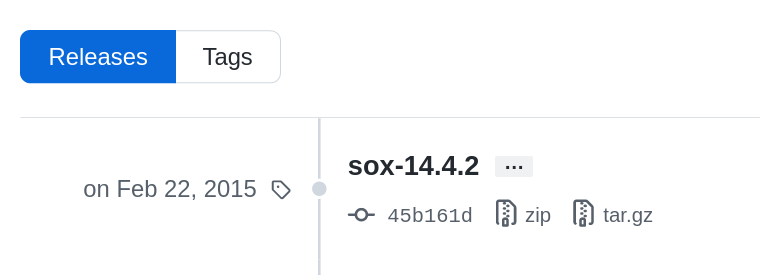
\includegraphics[width=0.8\textwidth]{sox-releases.png}

    \end{center}
\end{frame}

\begin{frame}[fragile]{}
    \frametitle{}
    \begin{center}
        \textbf{Development history}
        \vspace{0.2cm}

        \begin{flushleft}
        SoX has had several vulnerabilities listed in the National
        Vulnerability Database since its last public release in 2015. These
        vulnerabilities include stack and heap overflows and denial-of-service
        attacks.
        \end{flushleft}

    \end{center}
\end{frame}

\begin{frame}[fragile]{}
    \frametitle{}
    \begin{center}
        \textbf{Development history}
        \vspace{0.2cm}

        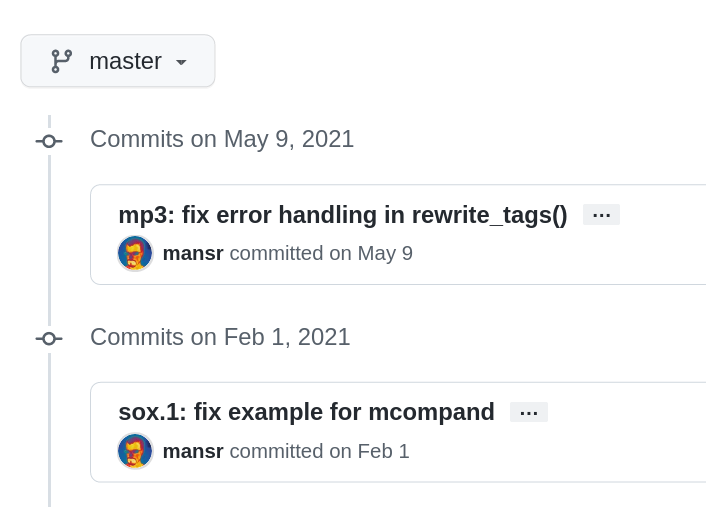
\includegraphics[width=0.7\textwidth]{sox-commits.png}

    \end{center}
\end{frame}

\fontsize{18pt}{18}\selectfont
\begin{frame}
  \vspace*{2.5cm}
  \begin{minipage}[b][\paperheight]{\textwidth}
  \begin{center}

      %\raggedright%
      \linespread{1.0}%
      \usebeamerfont{title}%
      \usebeamercolor[fg]{title}%
      \if@noSmallCapitals%
        Questions?
      \else%
        \scshape{\color{black} Questions?}%
      \fi%
      \vspace*{0.3em}

      \usebeamerfont{subtitle}%
      \fontsize{13pt}{14}\selectfont
      \usebeamercolor[fg]{subtitle}%
        \begin{itemize}[label={}]
            \item {\color{black} \twitter\ @erthalion}
            \item {\color{black} \email\ dmitrii.dolgov at zalando dot de}
            \item {\color{black} \email\ 9erthalion6 at gmail dot com}
        \end{itemize}
      \vspace*{2.5em}%

    \vfill
    \vspace*{2em}
  \end{center}
  \end{minipage}

\end{frame}

\end{document}
